\documentclass[11pt,a4paper]{article}
\usepackage[a4paper,margin=20mm,headheight=14pt]{geometry}
\usepackage[T1]{fontenc}
\usepackage{lmodern,amsmath,amssymb,booktabs,array,graphicx,xcolor,tikz,fancyhdr,hyperref,microtype}
\definecolor{ink}{HTML}{19334A}
\definecolor{muted}{HTML}{536477}
\hypersetup{colorlinks=true,linkcolor=ink,urlcolor=ink,pdftitle={Agentic VI: Variational difficulty profiling},pdfsubject={Working report v0.1, Tasks 001--003}}
\pagestyle{fancy}\fancyhf{}\lhead{\small\textcolor{muted}{AGENTIC VI / RESEARCH WORKING REPORT}}\rhead{\small\textcolor{muted}{v0.1}}
\lfoot{\small\textcolor{muted}{27 November 2026}}\rfoot{\small\textcolor{muted}{\thepage}}
\setlength{\parindent}{0pt}\setlength{\parskip}{5pt}
\setlength{\abovedisplayskip}{7pt}\setlength{\belowdisplayskip}{7pt}
\renewcommand{\arraystretch}{1.14}
\newcommand{\sectiontitle}[2]{\vspace*{1mm}{\large\bfseries\textcolor{muted}{#1}}\\[2pt]{\LARGE\bfseries\textcolor{ink}{#2}}\par\vspace{2mm}\hrule\vspace{3mm}}
\newcommand{\KL}{\operatorname{KL}}
\newcommand{\E}{\mathbb E}
\newcommand{\diag}{\operatorname{diag}}
\newcommand{\tr}{\operatorname{tr}}
\newcommand{\source}[1]{\par\smallskip{\footnotesize\textcolor{muted}{Source: #1}}\par}
\begin{document}
\thispagestyle{fancy}
{\small\bfseries\textcolor{muted}{WORKING REPORT \enspace / \enspace VERSION 0.1 \enspace / \enspace TASKS 001--003}}\\[4pt]
{\Huge\bfseries\textcolor{ink}{Agentic VI}}\\[5pt]
{\LARGE\bfseries Variational difficulty profiling with mean-field inference}\\[4pt]
{\large Preliminary mathematical framework and experimental evidence}\par
\vspace{2mm}\hrule\vspace{3mm}
\textbf{Abstract.} We investigate whether inexpensive mean-field variational inference (MFVI) can serve as a probe of inference difficulty, using only an unnormalized posterior density and its derivatives. A Variational Difficulty Profile (VDP) collects evidence about optimization, dependence, tail coverage, changing curvature and distinct fitted solutions from four independent MFVI runs. A protected computational budget accounts for all target evaluations. On Gaussian controls, the profile distinguishes several signs of incomplete optimization from persistent mean-field error. On the ten-dimensional Eight Schools posterior, the diagnostics favor non-centering at early matched budgets, consistent with independent quadrature-based posterior evaluation. These are controlled proof-of-concept results, not a calibrated decision policy or a general reliability guarantee.

\section*{1. Research objective and scope}
The long-term aim is to discover reliable VI algorithms that adapt objective, variational family, optimizer and parameterization to the problem. The current scope is narrower: Gaussian MFVI, reverse KL, Adam and a fixed diagnostic portfolio. The immediate question is whether the probe supplies useful information about \emph{why} inference is difficult, at a modest additional cost. The motivation includes robust stochastic VI optimization and high-dimensional VI \cite{dhaka20,dhaka21}. Reliability takes precedence over efficiency; complexity must be justified by evidence.

\textbf{Target-access contract.} For a proper target, write
\[p(x)=\tilde p(x)/Z,\qquad \ell(x)=\log\tilde p(x),\qquad Z=\int \tilde p(x)\,dx.\]
The inference algorithm receives dimension, an initialization policy and metered access to $\ell$, its score $g=\nabla\ell$ and Hessian-vector products. Known posterior moments, exact KL, target covariance and reference solutions are evaluator-only information. The additive constant in $\ell$ disappears from derivatives, normalized importance weights and same-target ELBO differences. For constrained models the coordinate transformation and its Jacobian are included in $\ell$.

\textbf{Milestones.}
\begin{center}\small
\begin{tabular}{p{17mm}p{61mm}p{77mm}}
\toprule Task & Scientific role & Status / evidence \\\midrule
001 & Analytical Gaussian baseline & 45 fits on nine fixed Gaussian targets \\
002 & Implement and validate VDP v0.1 & 39 profiles, 156 fits; Gaussian controls \\
003 & Test parameterization and changing geometry & Eight Schools, 8 profiles, 32 fits \\\bottomrule
\end{tabular}
\end{center}
This is a living research report, versioned as of 27 November 2026. Numerical findings are taken from archived repository reports and per-fit results, not newly rerun experiments. All claims are conditional on the tested targets, settings and coordinates. No autonomous discovery loop or calibrated difficulty score has yet been validated.
\source{\href{https://github.com/adhaka/agentic-vi/tree/research/003-eight-schools}{Agentic VI repository, Task 003 research branch}; \href{https://github.com/adhaka/agentic-vi/blob/main/VDP.md}{VDP v0.1 specification}.}
\newpage
\sectiontitle{METHODS / 02}{The variational probe and VDP}
\textbf{MFVI.} Let $q_\phi=\mathcal N(m,D)$, $D=\diag(s^2)$, $a=\log s$, and $x=m+s\odot\epsilon$, $\epsilon\sim\mathcal N(0,I)$. The unnormalized ELBO and pathwise ascent gradients are
\begin{align*}
L(\phi)&=\E_\epsilon[\ell(x)]+\sum_i a_i+\tfrac d2(1+\log 2\pi)=\log Z-\KL(q_\phi\|p),\\
\nabla_m L&=\E[g(x)],\qquad \nabla_a L=\mathbf1+\E[g(x)\odot s\odot\epsilon].
\end{align*}
Four dispersed starts use separate initialization and training random streams; diagnostic samples are independent of training. Task 002/003 use float64, constant-rate Adam ($0.03$), 64 draws/update, and a log-scale clamp $[-12,8]$. Horizons are 250, 500, 1,000 and 3,000 updates; histories are paired across horizons. A common-start control isolates stochastic-gradient variability.

\textbf{Structured profile.} The five elements are groups of measurements, not calibrated scalars:
\[\widehat{\mathbf C}=(C_{\rm opt},C_{\rm dep},C_{\rm tail},C_{\rm geom},C_{\rm mode}).\]
\begin{center}\small
\begin{tabular}{p{22mm}p{67mm}p{66mm}}
\toprule Component & Recorded evidence & Interpretation / limitation \\\midrule
$C_{\rm opt}$ & Classical and rank/folded split $\hat R$, drift, independent gradient mean and SE & Optimizer iterates, not posterior draws; no validated VI $\hat R$ cutoff \\
$C_{\rm dep}$ & Standardized off-diagonal curvature & Local interactions; not marginal correlation \\
$C_{\rm tail}$ & Pareto $\hat k$, raw and smoothed weight ESS & Finite-sample coverage warnings; missed regions may remain invisible \\
$C_{\rm geom}$ & Relative curvature variation and directional curvature & Local changing stiffness; not a global geometry certificate \\
$C_{\rm mode}$ & Six pairwise symmetric KL distances and within-run evidence & Distinct fits need not imply distinct posterior modes \\\bottomrule
\end{tabular}
\end{center}
\textbf{Optimization and weights.} For $M$ equal-length trajectories of length $n$, with within-chain variance $W$ and between-chain variance $B_R=n\operatorname{Var}(\bar x_m)$, classical $\hat R=\sqrt{[(n-1)W/n+B_R/n]/W}$. Rank normalization, splitting and folding follow \cite{vehtari21}; the last half of the logged iterates is used. Degenerate traces are flagged. Independent gradients are assessed in standardized coordinates $(s\odot g,1+s\odot\epsilon\odot g)$ with coordinate Monte Carlo SEs. Endpoint distances are $J_{ab}=\{\KL(q_a\|q_b)+\KL(q_b\|q_a)\}/2$, reported jointly and per dimension. With $x_j\sim q$, normalized weights are $w_j\propto\exp(\ell(x_j)-\log q(x_j))$, and $\mathrm{ESS}=1/\sum_j w_j^2$. PSIS is used as in \cite{yao18,vehtari24}. The sample-size reference $\min(1-1/\log_{10}S,0.7)$ is an importance-sampling warning, not a VI acceptance gate.

\textbf{Hard budget.} For $N_f$ values, $N_g$ gradients and $N_h$ HVPs, enforce $N_f+N_g+N_h\le B$ in target-evaluation-equivalent units (TEU). A value costs 1, value+gradient 2, and value+gradient+HVP 3 per point/direction. Reserve full batches before execution; failed attempts are charged, denied requests are not executed. This provisional convention is not a runtime equivalence. All pilot and diagnostic calls count; independent oracle evaluation does not enter the inference budget. The implementation isolates trusted components, not adversarial agents.
\newpage
\sectiontitle{METHODS / 03}{Matrix-free curvature and Gaussian validation}
\textbf{Curvature estimators.} Define $H(x)=-\nabla^2\ell(x)$ and $A(x)=D^{1/2}H(x)D^{1/2}$. At each of $J$ independent locations $x_j\sim q$, use the same $R$ independent Rademacher directions $z_r$ and compute $u_{jr}=A(x_j)z_r$ by metered HVPs. Let $t_{jri}=z_{ri}u_{jri}$. Conditional on the location, $\E_z t_{jri}=A_{ii}$ and $\operatorname{Var}_z(t_{jri})=\sum_{k\ne i}A_{ik}^2$. Thus total and off-diagonal squared Frobenius energies can be estimated without a dense Hessian:
\[F_j=\frac1R\sum_r\|u_{jr}\|^2,\quad O_j=\sum_i\widehat{\operatorname{Var}}_r(t_{jri}),\quad \widehat C_{\rm dep}=\sqrt{\frac{\sum_j O_j}{\sum_j F_j}}.\]
With $\bar u_r=J^{-1}\sum_j u_{jr}$, reuse the same HVPs for
\[V=\frac{1}{R(J-1)}\sum_{j,r}\|u_{jr}-\bar u_r\|^2,\qquad \widehat C_{\rm geom}=\sqrt{\frac{V}{J^{-1}\sum_j F_j}}.\]
The energy estimators are unbiased under the stated sampling and integrability assumptions, not their ratios. Values can exceed one at finite sample sizes; undefined denominators are flagged. Two-way bootstrap ranges describe exploratory sensitivity, not calibrated intervals. Curvature is parameterization-dependent and local to sampled $q$ support.

\textbf{Task 001: analytical baseline.} For $p=\mathcal N(\mu,\Sigma)$ with precision $P=\Sigma^{-1}$, reverse-KL optimal MFVI satisfies $m^*=\mu$, $v_i^*=1/P_{ii}$. The exact decomposition, with $r_i=P_{ii}v_i$, is
\begin{align*}
\KL(q\|p)&=\underbrace{\tfrac12(\log\det\Sigma+\sum_i\log P_{ii})}_{\text{family/objective floor}}\\[-1mm]
&\quad+\underbrace{\tfrac12[(m-\mu)^TP(m-\mu)+\sum_i(r_i-1-\log r_i)]}_{\text{optimization gap}}.
\end{align*}
The 45 runs (three geometries, dimensions 10/50/100, five seeds, 3,000 updates and 128 draws/update) demonstrate that convergence within a diagonal family is not sufficient for calibrated uncertainty. At $d=100$, the correlated and ill-conditioned floors account for 98.9\% and 99.1\% of mean KL, respectively.

\textbf{Task 002: normalization-free diagnostics.} The same nine archived matrices were used for 36 main profiles plus three controls, at four horizons with four dispersed runs. Selected final results ($d=100$, 3,000 updates):
\begin{center}\small
\begin{tabular}{lrrrrrr}
\toprule Target & Gap & Floor & Max $\hat R$ & Interaction & $\hat k$ & ESS \\\midrule
Independent & 0.205 & 0 & 1.03 & 0 & 0.153 & 673\\
Correlated & 0.284 & 22.3 & 1.05 & 0.556 & 1.82 & 1.66\\
Ill-conditioned & 0.685 & 72.3 & 2.51 & 0.834 & 3.06 & 1.64\\
\bottomrule
\end{tabular}
\end{center}
KL in joint nats; fit-level quantities are medians except profile maximum $\hat R$. ESS uses 1,024 draws. The ill-conditioned gap fell from 99.6 to 0.685 nats, while interaction was already 0.809 at 250 updates. Geometry was numerically zero throughout, as expected for Gaussian Hessians. A high-rate control produced nearly 12 times worse gap despite lower $\hat R$; trajectory stability is not accuracy. Diagnostic cost per profile was $8G+4S+12JR=7{,}680$ TEU for $G=256,S=1024,J=8,R=16$, 5.66\% of the shortest full budget.
\source{\href{https://github.com/adhaka/agentic-vi/blob/research/003-eight-schools/research/task001/REPORT.md}{Task 001 report}; \href{https://github.com/adhaka/agentic-vi/blob/research/003-eight-schools/research/task002/REPORT.md}{Task 002 report}.}
\newpage
\sectiontitle{EXPERIMENT / 04}{Eight Schools: model and reference}
The Eight Schools model has ten unconstrained coordinates but a hierarchical scale that induces nonlinear geometry. We use the standard data and the specified proper priors:
\[\mu\sim\mathcal N(0,25),\quad \tau\sim\operatorname{HalfCauchy}(5),\quad \theta_i\mid\mu,\tau\sim\mathcal N(\mu,\tau^2),\quad y_i\mid\theta_i\sim\mathcal N(\theta_i,\sigma_i^2).\]
\begin{center}\small
\begin{tabular}{lrrrrrrrr}\toprule School & 1&2&3&4&5&6&7&8\\\midrule
$y_i$&28&8&$-3$&7&$-1$&1&18&12\\
$\sigma_i$&15&10&16&11&9&11&10&18\\\bottomrule\end{tabular}
\end{center}
Write $\eta=\log\tau$, and let $z_i=(\theta_i-\mu)/\tau$. Up to the same additive constants, the centered (CP) and non-centered (NCP) log densities in their respective coordinates are
\begin{align*}
\ell_C&=-\mu^2/50-\log(1+e^{2\eta}/25)-7\eta
-\tfrac12 e^{-2\eta}\sum_i(\theta_i-\mu)^2
-\tfrac12\sum_i (y_i-\theta_i)^2/\sigma_i^2,\\
\ell_N&=-\mu^2/50-\log(1+e^{2\eta}/25)+\eta
-\tfrac12\sum_i z_i^2
-\tfrac12\sum_i(y_i-\mu-e^\eta z_i)^2/\sigma_i^2.
\end{align*}
Both include the scale Jacobian; $\ell_N=\ell_C+8\eta$ at corresponding points. The centered school-coordinate curvature is $\tau^{-2}+\sigma_i^{-2}$, versus $1+\tau^2/\sigma_i^2$ for NCP. The former diverges near $\tau=0$; non-centering alleviates that part of the funnel but retains likelihood coupling.

\textbf{Independent reference.} After integrating out $\theta$, $y_i\mid\mu,t\sim\mathcal N(\mu,\sigma_i^2+t^2)$. For $w_i=(\sigma_i^2+t^2)^{-1}$, $V=(1/25+\sum_i w_i)^{-1}$ and $m=V\sum_iw_i y_i$, the conditional population mean is $\mu\mid t,y\sim\mathcal N(m,V)$. Integrating $\mu$ gives $y\mid t\sim\mathcal N(0,\diag(\sigma_i^2+t^2)+25\mathbf1\mathbf1^T)$. Gauss--Legendre integration in the half-Cauchy prior probability coordinate $u=(2/\pi)\arctan(t/5)$ yields the reference. For $b_i=t^2/(t^2+\sigma_i^2)$, conditional school moments are $b_i y_i+(1-b_i)m$ and $b_i\sigma_i^2+(1-b_i)^2V$. Integrating moments and conditional CDFs gives scientific-coordinate summaries. The reference log evidence is $-31.31134735229279$; refinement (128 to 256 nodes) changed marginal summaries by at most $5.4\times10^{-14}$; a separate adaptive integral agreed in log evidence within $4\times10^{-15}$.

\textbf{Design.} Two parameterizations, four horizons, four runs per profile; no new diagnostic or optimizer. Identical numeric initialization policies and paired random draws do not imply identical starting distributions in scientific coordinates. The attainable mean-field families also differ after transformation. The comparison therefore measures the combined effect of parameterization, family and initialization, not an isolated optimizer effect. The evaluator uses normalized joint densities and analytic Gaussian/lognormal expectations plus scalar quadrature for reverse KL and transformed quantiles. No reference information enters inference.
\begin{center}\small
\begin{tabular}{lrrrr}\toprule Updates & 250 & 500 & 1,000 & 3,000\\\midrule TEU per profile &135,680&263,680&519,680&1,543,680\\\bottomrule\end{tabular}
\end{center}
\source{\href{https://github.com/adhaka/agentic-vi/blob/research/003-eight-schools/research/task003/PROTOCOL.md}{Frozen Task 003 protocol}; \href{https://github.com/adhaka/agentic-vi/blob/research/003-eight-schools/research/task003/REPORT.md}{Task 003 report}.}
\newpage
\sectiontitle{RESULTS / 05}{Eight Schools: diagnostic evidence}
The non-centered fit had lower reverse KL in every one of the 16 paired comparisons (not 16 independent replications). Differences are visible at 250 updates. The table summarizes the observed profile values; no thresholds were fitted.
\begin{center}\small
\begin{tabular}{lrrrrrrrr}\toprule Form & Steps & KL & Pair max & $\hat R_{\max}$ & Geometry & Depend. & $\hat k$ & ESS\\\midrule
CP &250&7.141&37.70&4.61&0.897&0.614&1.020&30.5\\
NCP&250&0.326&0.416&3.40&0.521&0.336&0.661&399\\
CP &500&5.900&34.00&4.58&0.859&0.612&0.863&24.1\\
NCP&500&0.307&0.109&2.38&0.257&0.219&0.502&429\\
CP &1,000&4.681&23.42&4.55&0.820&0.623&1.178&6.42\\
NCP&1,000&0.331&0.135&1.38&0.263&0.250&0.527&219\\
CP &3,000&2.447&9.84&3.89&0.691&0.612&0.797&23.9\\
NCP&3,000&0.323&0.100&1.07&0.398&0.328&0.616&354\\\bottomrule
\end{tabular}
\end{center}
{\footnotesize Fit-dependent entries are four-run medians; pair max and $\hat R_{\max}$ are profile maxima. KL and pair max are joint nats; ESS is raw importance ESS out of 1,024. KL is evaluator-only.}\par
\begin{center}
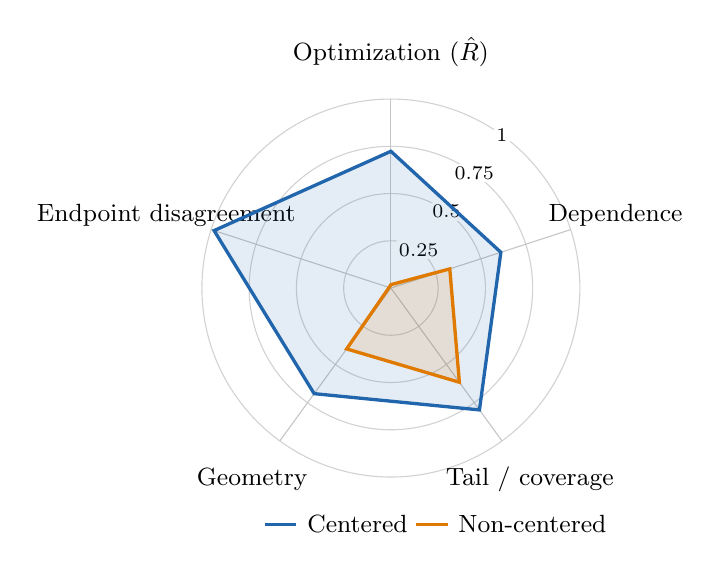
\begin{tikzpicture}[scale=0.80, font=\small]
\definecolor{cpblue}{HTML}{2166AC}\definecolor{ncporange}{HTML}{DF7900}
\foreach \r in {0.25,0.5,0.75,1}{\draw[gray!35] (0,0) circle ({3*\r});}
\foreach \a/\lab in {90/{Optimization ($\hat R$)},18/{Dependence},-54/{Tail / coverage},-126/{Geometry},162/{Endpoint disagreement}}{
\draw[gray!45] (0,0)--(\a:3);\node[align=center] at (\a:3.75) {\lab};}
\foreach \r in {0.25,0.5,0.75,1}{\node[font=\scriptsize,fill=white,inner sep=1pt] at (54:{3*\r}) {\r};}
\filldraw[fill=cpblue,fill opacity=.12,draw=cpblue,very thick] (90:2.1707)--(18:1.8354)--(-54:2.3915)--(-126:2.0728)--(162:2.9512)--cycle;
\filldraw[fill=ncporange,fill opacity=.13,draw=ncporange,very thick] (90:.0538)--(18:.9830)--(-54:1.8491)--(-126:1.1946)--(162:.0300)--cycle;
\draw[cpblue,very thick] (-2,-3.75)--(-1.5,-3.75) node[right,black]{Centered};
\draw[ncporange,very thick] (.4,-3.75)--(.9,-3.75) node[right,black]{Non-centered};
\end{tikzpicture}\par
{\small\textbf{Figure 1.} Final-horizon radar visualization using the archived summary values. The radii are $(\hat R_{\max}-1)/4$, dependence, $\hat k$, geometry, and pair max/10 nats (clipped to $[0,1]$ if needed). Axis-specific scales are illustrative, not calibrated; area has no quantitative meaning. Endpoint disagreement is not evidence sufficient to establish posterior multimodality.}
\end{center}
The early NCP KL (0.326 nats) is smaller than final CP KL (2.447), and the median curvature measures favor NCP at all horizons. At the final horizon one NCP fit nevertheless had geometry 0.825, overlapping centered fits. The diagnostics are therefore useful group-level evidence, not a deterministic ranking of individual fits.
\source{\href{https://github.com/adhaka/agentic-vi/blob/research/003-eight-schools/research/task003/evaluation/per_fit.csv}{Task 003 per-fit data}; \href{https://github.com/adhaka/agentic-vi/blob/research/003-eight-schools/research/task003/evaluation/vdp_radar.svg}{repository radar figure}.}
\newpage
\sectiontitle{SYNTHESIS / 06}{What we know, and what remains open}
\textbf{Scientific-coordinate accuracy.} At 3,000 updates, median fitted summaries show improved population mean and uncertainty under non-centering, but both variants miss parts of the scale distribution.
\begin{center}\small
\begin{tabular}{lrrr}\toprule Quantity & Reference & CP & NCP\\\midrule
$\mu$ mean &4.397&1.990&4.487\\
$\mu$ SD &3.318&1.578&3.141\\
$\tau$ 5th percentile &0.246&3.431&0.698\\
$\tau$ 95th percentile &9.842&7.667&7.373\\
School mean MAE &--&2.368&0.381\\
School SD MAE &--&0.589&0.322\\\bottomrule\end{tabular}
\end{center}
The centered scale upper quantile is slightly closer to the reference. Between 500 and 3,000 updates NCP maximum $\hat R$ drops from 2.38 to 1.07 while median KL rises from 0.307 to 0.323. In one final paired run, CP has better importance ESS and $\hat k$ but worse joint KL (2.182 versus 0.327). Across all 16 comparisons, independent MC ELBO also favors NCP in 16, curvature variation in 15, ESS in 15 and $\hat k$ in 14. A key open question is the incremental value of VDP beyond the ELBO, which already ranks these fits well.

\textbf{Computational record and evidence limits.} Task 001 used 17.28 million training draws (historical accounting); Task 002 used 22,446,080 TEU in the main study plus 5,648 smoke TEU; Task 003 used 4,925,440 TEU, including 2,477,056 values, 2,444,288 gradients and 4,096 HVPs. Task 003 reported 21 passing tests, no denied or failed calls and 19.81 s inference driver time after imports on one CPU thread. These are reported run records, not timings or test results independently reproduced for this document. Task 002's analytic Gaussian provider is not a timing comparator for the PyTorch autodiff backend. The Gaussian experiments have only one instance per cell; Eight Schools has one dataset and prior. No estimate of across-instance diagnostic reliability is available. Local samples may miss remote modes, and bootstrap sensitivity ranges are uncalibrated. The historical rotated covariance generator used rank-deficient sine inputs; archived realized matrices preserve reproducibility. Extreme finite inputs can still require numerical safeguards.

\textbf{Next milestone (proposed, not authorized experiments).} Consolidate Tasks 001--003 and retain the frozen five-component profile. Before broadening the family or objective, assess whether the existing signals justify their computational cost and add actionable information beyond ELBO and simple restart agreement. Use a small, preregistered comparison with meaningful quality criteria when proceeding. No new diagnostic, automatic intervention policy or universal score is proposed here. The candidate contribution is a budgeted diagnostic framework whose predictive usefulness must be validated, not novelty of individual established diagnostics.

\begingroup\small
\begin{thebibliography}{9}\setlength{\itemsep}{1pt}\setlength{\parskip}{0pt}
\bibitem{dhaka20} Dhaka et al. Robust, Accurate Stochastic Optimization for Variational Inference. NeurIPS, 2020.
\bibitem{dhaka21} Dhaka et al. Challenges and Opportunities in High Dimensional Variational Inference. NeurIPS, 2021.
\bibitem{vehtari21} Vehtari et al. Rank-normalization, folding, and localization: An improved $\hat R$ for assessing convergence of MCMC. Bayesian Analysis, 2021.
\bibitem{yao18} Yao, Vehtari, Simpson and Gelman. Yes, but Did It Work?: Evaluating Variational Inference. ICML, 2018.
\bibitem{vehtari24} Vehtari et al. Pareto Smoothed Importance Sampling. JMLR, 2024.
\end{thebibliography}\endgroup
\end{document}
